\section{Algoritma Uniform Cost Search (UCS)}

Uniform Cost Search (UCS) adalah algoritma pencarian yang mengembangkan node dengan biaya jalur terkecil $g(n)$ terlebih dahulu. UCS menjamin menemukan solusi dengan total biaya minimum apabila semua biaya tepi bernilai tidak negatif, karena selalu memilih state dengan $g$ terkecil untuk diekspansi \cite{dijkstra1959note,russell2010artificial}. Beberapa sifat penting UCS adalah sebagai berikut.
\begin{itemize}
    \item \textbf{Optimalitas}. UCS optimal jika biaya tiap langkah non-negatif.
    \item \textbf{Keterlengkapan}. UCS akan menemukan solusi apabila ruang status berhingga dan ada path menuju tujuan.
    \item \textbf{Kompleksitas}. Bergantung pada branching factor dan distribusi biaya. Pada kasus terburuk dapat menimbulkan eksplorasi besar jika banyak node memiliki biaya jalur serupa.
\end{itemize}

\subsection{Definisi $f(n)$ dan $g(n)$ untuk UCS}
Dalam implementasi solver Ice Sliding Puzzle ini, definisi fungsi biaya yang digunakan adalah sebagai berikut.
\begin{itemize}
    \item $g(n)$: total biaya kumulatif dari semua gerakan yang dilakukan dari keadaan awal sampai mencapai node/state $n$. Untuk setiap gerakan sliding, biaya gerakan adalah jumlah cost dari tiap tile yang dilalui selama sliding (catatan: tile posisi awal sebelum sliding tidak dihitung, tetapi tile tempat aktor berhenti dihitung).
    \item $f(n)$: untuk UCS, kita menggunakan $f(n)=g(n)$. Prioritas antrian eksplorasi didasarkan pada nilai $g(n)$ terkecil.
\end{itemize}

\subsection{Implementasi UCS pada Kode Sumber}
Berdasarkan implementasi di \texttt{src/core/search/Search.cpp}, UCS dijalankan melalui fungsi umum \texttt{Search::solve} dengan aturan prioritas \texttt{computePriority = gCost}. State direpresentasikan sebagai triple \texttt{(row, col, nextCheckpoint)}. Di bawah ini adalah uraian langkah demi langkah yang merepresentasikan apa yang dilakukan kode pada setiap tahap.

\begin{enumerate}
    \item \textbf{Inisialisasi state awal}: buat node awal dengan posisi start, \texttt{nextCheckpoint=0}, \texttt{g=0}, dan hitung heuristik (meskipun untuk UCS heuristik tidak dipakai untuk prioritas, nilai h biasanya disimpan untuk konsistensi struktur node).
    \item \textbf{Siapkan frontier}: buat \texttt{priority\_queue} (disebut \texttt{frontier}) yang mengurutkan node menurut prioritas; untuk UCS prioritas ini adalah \texttt{gCost}.
    \item \textbf{Best-cost map}: buat \texttt{unordered\_map<StateKey,int>} bernama \texttt{bestCost} untuk menyimpan biaya terbaik (terkecil) yang pernah ditemukan untuk setiap state (key = posisi + nextCheckpoint).
    \item \textbf{Masukkan start}: push node awal ke \texttt{frontier} dan set \texttt{bestCost[start.state] = 0}.
    \item \textbf{Main loop}: selama \texttt{frontier} tidak kosong, ambil node dengan prioritas terkecil (pop): ini adalah node dengan \texttt{g} terkecil pada saat itu.
    \item \textbf{Pruning cepat}: jika node yang di-pop memiliki \texttt{g > bestCost[state]} berarti ada jalur lebih baik yang sudah dicatat -> lewati node tersebut (continue).
    \item \textbf{Cek goal}: periksa apakah node memenuhi kondisi goal (posisi = goal dan \texttt{nextCheckpoint > maxCheckpoint}). Jika ya, lakukan rekonstruksi jalur (backtrack menggunakan \texttt{parentIndex}) dan kembalikan hasil.
    \item \textbf{Generate successor}: untuk setiap arah gerak (Up/Down/Left/Right) panggil \texttt{rules.applyMove(board, current.pos, current.nextCheckpoint, dir)}. Fungsi ini meng-"slide" aktor sampai berhenti, mengakumulasi biaya tile yang dilalui, dan mengembalikan posisi akhir, biaya gerak serta nilai \texttt{nextCheckpoint} baru bila melewati checkpoint.
    \item \textbf{Filter outcome tidak valid}: jika hasil \texttt{applyMove} menyatakan \texttt{outOfBounds}, \texttt{hitLava}, atau gerakan invalid lainnya, abaikan successor tersebut.
    \item \textbf{Hitung biaya kumulatif}: untuk setiap successor valid, hitung \texttt{next.g = current.g + outcome.moveCost} dan bentuk \texttt{next.state = (outcome.end, outcome.nextCheckpoint)}.
    \item \textbf{Pruning berdasarkan bestCost}: jika \texttt{bestCost[next.state]} ada dan \texttt{next.g >= bestCost[next.state]}, abaikan successor (jalur lebih mahal atau sama sudah ada). Jika lebih baik, set \texttt{bestCost[next.state] = next.g}.
    \item \textbf{Enqueue}: masukkan successor ke \texttt{frontier} dengan prioritas \texttt{next.g}. Simpan indeks parent untuk rekonstruksi jalur.
\end{enumerate}

\begin{algorithm}[H]
    \caption{Uniform Cost Search (UCS) pada Solver}
    \begin{algorithmic}[1]
        \Require \textit{board}, \textit{rules}
        \Ensure \textit{SearchResult}
        \State $start \gets (board.start, nextCheckpoint=0, g=0)$
        \State $frontier \gets$ priority queue terurut naik berdasarkan $g$
        \State masukkan $start$ ke $frontier$
        \State $bestCost[(start.pos, start.nextCheckpoint)] \gets 0$
        \While{$frontier$ tidak kosong}
        \State $current \gets pop(frontier)$
        \If{$current.g > bestCost[current.state]$}
        \State \textbf{continue}
        \EndIf
        \If{$isGoalState(current.pos, current.nextCheckpoint)$}
        \State \Return $reconstructPath(current)$
        \EndIf
        \For{setiap $dir \in \{Up, Down, Left, Right\}$}
        \State $outcome \gets applyMove(board, current.pos, current.nextCheckpoint, dir)$
        \If{$outcome.invalid$ \textbf{or} $outcome.hitLava$ \textbf{or} $outcome.outOfBounds$}
        \State \textbf{continue}
        \EndIf
        \State $next.g \gets current.g + outcome.moveCost$
        \State $next.state \gets (outcome.end, outcome.nextCheckpoint)$
        \If{$outcome.end = board.goal$ \textbf{and} $outcome.nextCheckpoint \le board.maxCheckpoint$}
        \State \textbf{continue}
        \EndIf
        \If{$next.state \in bestCost$ \textbf{and} $next.g \ge bestCost[next.state]$}
        \State \textbf{continue}
        \EndIf
        \State $bestCost[next.state] \gets next.g$
        \State masukkan $next$ ke $frontier$ dengan prioritas $next.g$
        \EndFor
        \EndWhile
        \State \Return \textit{failure}
    \end{algorithmic}
\end{algorithm}

\subsection{Contoh Pencarian UCS}
Sebagai ilustrasi, misalkan terdapat graf pencarian sederhana berikut. Angka di dalam kurung menunjukkan biaya kumulatif $g(n)$.

\begin{figure}[H]
    \centering
    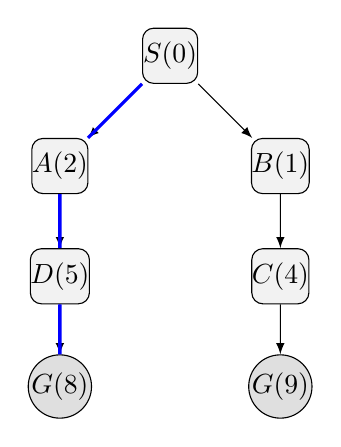
\begin{tikzpicture}[
            level distance=14mm,
            sibling distance=28mm,
            every node/.style={draw, circle, minimum size=7mm, inner sep=0pt},
            chosen/.style={draw, circle, fill=gray!25, minimum size=7mm, inner sep=0pt},
            edge from parent/.style={draw, -latex}
        ]
        \node[draw, rectangle, rounded corners, fill=gray!10] (S) {$S(0)$}
        child { node[draw, rectangle, rounded corners, fill=gray!10] (A) {$A(2)$}
                child { node[draw, rectangle, rounded corners, fill=gray!10] (D) {$D(5)$}
                        child { node[chosen] (G1) {$G(8)$} }
                    }
            }
        child { node[draw, rectangle, rounded corners, fill=gray!10] (B) {$B(1)$}
                child { node[draw, rectangle, rounded corners, fill=gray!10] (C) {$C(4)$}
                        child { node[chosen] (G2) {$G(9)$} }
                    }
            };
        \draw[very thick, blue] (S) -- (A) -- (D) -- (G1);
    \end{tikzpicture}
    \caption{Contoh pohon pencarian UCS. Jalur terpilih adalah $S \rightarrow A \rightarrow D \rightarrow G$ karena memiliki biaya kumulatif minimum pada setiap ekspansi.}
    \label{fig:contoh-ucs}
\end{figure}

Pada contoh ini, urutan rute yang dipilih adalah $S \rightarrow A \rightarrow D \rightarrow G$. UCS selalu memilih node dengan $g(n)$ terkecil, sehingga meskipun ada cabang lain yang tampak lebih pendek secara langkah, jalur dengan biaya kumulatif paling kecil tetap diprioritaskan.

\section{Algoritma Greedy Best-First Search (GBFS)}

Greedy Best-First Search (GBFS) merupakan algoritma pencarian yang memilih node untuk diekspansi berdasarkan nilai heuristik $h(n)$ saja, yakni node yang dianggap paling "dekat" ke tujuan menurut heuristik. GBFS tidak mempertimbangkan biaya jalur $g(n)$ sehingga dapat menjadi sangat cepat namun tidak menjamin optimalitas atau keterlengkapan dalam semua kasus \cite{russell2010artificial}. Karakteristik GBFS dapat dijabarkan sebagai berikut.
\begin{itemize}
    \item \textbf{Kecepatan}. Seringkali lebih cepat menemukan solusi dibanding pencarian yang mempertimbangkan $g(n)$, terutama bila heuristik sangat informatif.
    \item \textbf{Non-optimal}. GBFS tidak menjamin menemukan solusi dengan biaya minimal.
    \item \textbf{Sensitif terhadap heuristik}. kualitas heuristik sangat menentukan performa dan hasil pencarian.
\end{itemize}

\subsection{Definisi $f(n)$ dan $g(n)$ untuk GBFS}
Untuk GBFS pada solver ini berlaku
\begin{itemize}
    \item $g(n)$: sama seperti pada UCS, dapat dihitung sebagai total biaya kumulatif sampai node $n$, namun nilai ini \emph{tidak} digunakan untuk menentukan urutan ekspansi.
    \item $f(n)$: GBFS menggunakan $f(n)=h(n)$, yaitu hanya mengurutkan node menurut estimasi heuristik menuju tujuan. Dengan demikian antrian prioritas berdasarkan $h(n)$ saja.
\end{itemize}

\subsection{Implementasi GBFS pada Kode Sumber}
Pada kode sumber yang sama, GBFS tidak membuat fungsi terpisah; perbedaannya hanya pada prioritas antrian: \texttt{computePriority = hCost}. Nilai heuristik dihitung oleh \texttt{Heuristic::estimate} (\texttt{src/core/heuristic/Heuristic.cpp}) sesuai pilihan \texttt{HeuristicType}. Di bawah ini alur langkah demi langkah implementasi GBFS dalam kode.

\begin{enumerate}
    \item \textbf{Inisialisasi}: buat node awal dengan \texttt{g=0} dan hitung \texttt{h = Heuristic::estimate(...)} untuk posisi awal.
    \item \textbf{Frontier}: buat \texttt{priority\_queue} yang mengurutkan node berdasarkan nilai heuristik \texttt{h} (nilai lebih kecil = prioritas lebih tinggi).
    \item \textbf{Best-cost map}: seperti UCS, tetap gunakan \texttt{bestCost} untuk menyimpan \texttt{g} terbaik yang ditemukan untuk setiap state. Ini membantu menghindari revisits yang jelas lebih mahal.
    \item \textbf{Masukkan start}: push node awal ke frontier dengan prioritas \texttt{start.h}.
    \item \textbf{Main loop}: pop node dengan \texttt{h} terkecil.
    \item \textbf{Pruning}: jika \texttt{current.g > bestCost[current.state]} maka lewati.
    \item \textbf{Cek goal}: jika memenuhi kondisi goal, rekonstruksi dan kembalikan jalur.
    \item \textbf{Generate successor}: untuk tiap arah, panggil \texttt{rules.applyMove} untuk mendapatkan posisi akhir dan \texttt{moveCost} sama seperti pada UCS.
    \item \textbf{Validasi}: tolak successor yang outOfBounds, hitLava, atau invalid.
    \item \textbf{Kalkulasi g dan h}: hitung \texttt{next.g = current.g + outcome.moveCost} dan \texttt{next.h = Heuristic::estimate(..., outcome.end, outcome.nextCheckpoint)}.
    \item \textbf{Pruning bestCost}: jika ada entri \texttt{bestCost[next.state]} yang lebih baik, abaikan; jika lebih baik, perbarui \texttt{bestCost[next.state] = next.g}.
    \item \textbf{Enqueue}: push successor ke frontier dengan prioritas \texttt{next.h}. Simpan parent index untuk rekonstruksi.
\end{enumerate}

Catatan implementasi khusus GBFS di kode:
\begin{itemize}
    \item Meski prioritas adalah heuristik, penyimpanan \texttt{g} dan penggunaan \texttt{bestCost} membantu menghindari eksplorasi ulang yang jelas lebih mahal.
    \item Performa sangat bergantung pada kualitas heuristik: heuristik yang informatif mengarahkan eksplorasi ke goal dengan cepat.
\end{itemize}

\begin{algorithm}[H]
    \caption{Greedy Best-First Search (GBFS) pada Solver}
    \begin{algorithmic}[1]
        \Require \textit{board}, \textit{rules}, \textit{heuristicType}
        \Ensure \textit{SearchResult}
        \State $start.g \gets 0$
        \State $start.h \gets estimate(board, start.pos, start.nextCheckpoint, heuristicType)$
        \State $frontier \gets$ priority queue terurut naik berdasarkan $h$
        \State masukkan $start$ ke $frontier$ dengan prioritas $start.h$
        \State $bestCost[(start.pos, start.nextCheckpoint)] \gets 0$
        \While{$frontier$ tidak kosong}
        \State $current \gets pop(frontier)$
        \If{$current.g > bestCost[current.state]$}
        \State \textbf{continue}
        \EndIf
        \If{$isGoalState(current.pos, current.nextCheckpoint)$}
        \State \Return $reconstructPath(current)$
        \EndIf
        \For{setiap $dir \in \{Up, Down, Left, Right\}$}
        \State $outcome \gets applyMove(board, current.pos, current.nextCheckpoint, dir)$
        \If{$outcome.invalid$ \textbf{or} $outcome.hitLava$ \textbf{or} $outcome.outOfBounds$}
        \State \textbf{continue}
        \EndIf
        \State $next.g \gets current.g + outcome.moveCost$
        \State $next.h \gets estimate(board, outcome.end, outcome.nextCheckpoint, heuristicType)$
        \State $next.state \gets (outcome.end, outcome.nextCheckpoint)$
        \If{$outcome.end = board.goal$ \textbf{and} $outcome.nextCheckpoint \le board.maxCheckpoint$}
        \State \textbf{continue}
        \EndIf
        \If{$next.state \in bestCost$ \textbf{and} $next.g \ge bestCost[next.state]$}
        \State \textbf{continue}
        \EndIf
        \State $bestCost[next.state] \gets next.g$
        \State masukkan $next$ ke $frontier$ dengan prioritas $next.h$
        \EndFor
        \EndWhile
        \State \Return \textit{failure}
    \end{algorithmic}
\end{algorithm}

\subsection{Contoh Pencarian GBFS}
Misalkan heuristik yang digunakan memberi estimasi jarak ke tujuan seperti nilai di bawah ini. Angka dalam kurung adalah $h(n)$.

\begin{figure}[H]
    \centering
    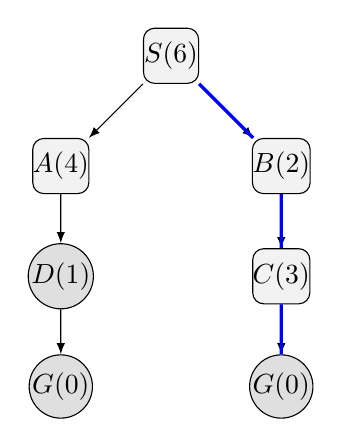
\begin{tikzpicture}[
            level distance=14mm,
            sibling distance=28mm,
            every node/.style={draw, circle, minimum size=7mm, inner sep=0pt},
            chosen/.style={draw, circle, fill=gray!25, minimum size=7mm, inner sep=0pt},
            edge from parent/.style={draw, -latex}
        ]
        \node[draw, rectangle, rounded corners, fill=gray!10] (S) {$S(6)$}
        child { node[draw, rectangle, rounded corners, fill=gray!10] (A) {$A(4)$}
                child { node[chosen] (D) {$D(1)$}
                        child { node[chosen] (G1) {$G(0)$} }
                    }
            }
        child { node[draw, rectangle, rounded corners, fill=gray!10] (B) {$B(2)$}
                child { node[draw, rectangle, rounded corners, fill=gray!10] (C) {$C(3)$}
                        child { node[chosen] (G2) {$G(0)$} }
                    }
            };
        \draw[very thick, blue] (S) -- (B) -- (C) -- (G2);
    \end{tikzpicture}
    \caption{Contoh pohon pencarian GBFS. Jalur terpilih adalah $S \rightarrow B \rightarrow C \rightarrow G$ karena node-node pada cabang ini memiliki nilai heuristik paling kecil.}
    \label{fig:contoh-gbfs}
\end{figure}

Pada contoh ini, GBFS memilih node dengan nilai heuristik terkecil terlebih dahulu, sehingga jalur yang diambil tidak selalu jalur termurah. Fokus utamanya adalah mendekati tujuan secepat mungkin menurut estimasi heuristik.

\section{Algoritma A$^\ast$}

A$^\ast$ (A-star) merupakan algoritma \textit{Pathfinding} yang menggabungkan keuntungan UCS dan heuristik dengan menggunakan fungsi evaluasi
$$f(n) = g(n) + h(n),$$

untuk melakukan memilih path dengan cost paling minumum. Dalam hal ini, $g(n)$ adalah biaya jalur dari root ke node $n$ dan $h(n)$ adalah heuristik estimasi biaya dari $n$ ke tujuan. A$^\ast$ bersifat optimal jika heuristik $h$ adalah \emph{admissible} (tidak melebihkan cost sebenarnya) dan akan efisien apabila $h$ juga \emph{consistent} (monotonik) \cite{hart1968formal,russell2010artificial}. Sifat-sifat A$^\ast$ adalah sebagai berikut.
\begin{itemize}
    \item \textbf{Optimalitas}. Terjamin bila $h$ admissible.
    \item \textbf{Efisiensi}. Jumlah node yang diekspansi seminimal mungkin di antara semua algoritma yang menggunakan heuristik yang sama dan tetap optimal.
    \item \textbf{Ketergantungan heuristik}. Heuristik yang lebih informatif (mendekati nilai cost sebenarnya) akan mengurangi ruang pencarian.
\end{itemize}

\subsection{Definisi $f(n)$ dan $g(n)$ untuk A$^\ast$}
Pada A$^\ast$ yang diimplementasikan untuk Ice Sliding Puzzle adalah sebagai berikut.
\begin{itemize}
    \item $g(n)$: sama dengan UCS, total biaya kumulatif dari seluruh gerakan sampai node $n$, dengan tiap gerakan bernilai jumlah cost tile yang dilintasi selama sliding.
    \item $f(n)$: $f(n)=g(n)+h(n)$ di mana $h(n)$ adalah heuristik estimasi biaya tersisa. Untuk memastikan A$^\ast$ tetap optimal, pilih heuristik yang \emph{admissible}. Contoh heuristik admissible yang sering dipakai pada grid-based sliding problems adalah
          $$h(n) = d_{manhattan}(pos(n), goal) \times c_{min},$$
          di mana $d_{manhattan}$ adalah jarak Manhattan antara posisi berhenti aktor pada state $n$ dan posisi tujuan, dan $c_{min}$ adalah lower bound dari cost tiap tile pada instance (mis. nilai minimal dari matriks cost). Karena setiap langkah sliding setidaknya akan menempuh jarak fisik minimal dan setiap tile memiliki biaya tidak kurang dari $c_{min}$, heuristik ini tidak melebihkan biaya sebenarnya sehingga admissible.
\end{itemize}

\subsection{Implementasi A$^\ast$ pada Kode Sumber}
A$^\ast$ juga berbagi kerangka yang sama di \texttt{Search::solve}, tetapi prioritasnya menggunakan jumlah biaya aktual dan heuristik: \texttt{computePriority = gCost + hCost}. Di bawah ini langkah demi langkah yang persis tercermin di implementasi kode.

\begin{enumerate}
    \item \textbf{Inisialisasi node awal}: buat node awal dengan \texttt{g=0} dan hitung \texttt{h = Heuristic::estimate(...)} berdasarkan \texttt{HeuristicType} yang dipilih.
    \item \textbf{Frontier}: buat \texttt{priority\_queue} yang mengurutkan node berdasarkan nilai \texttt{f = g + h} (nilai lebih kecil = prioritas lebih tinggi). Comparator di kode juga menerapkan tie-breaker tambahan (mis. prioritas, lalu \texttt{gCost}, lalu urutan masuk) untuk determinisme.
    \item \textbf{Best-cost map}: buat atau gunakan \texttt{bestCost} untuk menyimpan \texttt{g} terbaik per state. Ini memastikan kita tidak memproses jalur yang jelas lebih mahal.
    \item \textbf{Masukkan start}: push node awal ke frontier dengan prioritas \texttt{start.g + start.h}.
    \item \textbf{Main loop}: pop node dengan fungsi evaluasi \texttt{f} terkecil.
    \item \textbf{Pruning cepat}: jika \texttt{current.g > bestCost[current.state]} lewati node.
    \item \textbf{Cek goal}: jika kondisi goal terpenuhi (posisi = goal dan semua checkpoint telah dilewati), rekonstruksi jalur dan kembalikan hasil.
    \item \textbf{Generate successor}: panggil \texttt{rules.applyMove} untuk tiap arah gerak. Fungsi ini memberikan posisi akhir, biaya gerak, dan update \texttt{nextCheckpoint} jika checkpoint dilintasi.
    \item \textbf{Validasi outcome}: abaikan successor jika \texttt{outcome.invalid}, \texttt{outcome.hitLava}, atau \texttt{outcome.outOfBounds}.
    \item \textbf{Kalkulasi g, h, f}: hitung \texttt{next.g = current.g + outcome.moveCost}, lalu \texttt{next.h = Heuristic::estimate(..., outcome.end, outcome.nextCheckpoint)}; prioritas yang akan dimasukkan adalah \texttt{next.f = next.g + next.h}.
    \item \textbf{Pruning bestCost}: jika sudah ada \texttt{bestCost[next.state]} dengan nilai lebih kecil atau sama, abaikan; jika lebih kecil, perbarui entry tersebut.
    \item \textbf{Enqueue}: push successor ke frontier dengan prioritas \texttt{next.f} dan simpan parent untuk rekonstruksi.
\end{enumerate}

Catatan implementasi penting:
\begin{itemize}
    \item \texttt{StateKey} yang memuat \texttt{nextCheckpoint} membuat posisi yang sama dengan progres berbeda menjadi state berbeda  ini penting untuk permasalahan checkpoint ordering.
    \item Pruning pada \texttt{bestCost} menggunakan \texttt{gCost} menjaga agar A$^\ast$ tidak memproses jalur yang lebih mahal menuju state yang sama, sekaligus kompatibel dengan heuristik admissible untuk memastikan optimalitas.
    \item Penentuan nilai heuristik (admissible vs.
          informed) menentukan apakah A$^\ast$ yang berjalan akan optimal dan seberapa efisien ia akan memotong ruang pencarian.
\end{itemize}

\begin{algorithm}[H]
    \caption{A* Search pada Solver}
    \begin{algorithmic}[1]
        \Require \textit{board}, \textit{rules}, \textit{heuristicType}
        \Ensure \textit{SearchResult}
        \State $start.g \gets 0$
        \State $start.h \gets estimate(board, start.pos, start.nextCheckpoint, heuristicType)$
        \State $frontier \gets$ priority queue terurut naik berdasarkan $(g+h)$
        \State masukkan $start$ ke $frontier$ dengan prioritas $start.g + start.h$
        \State $bestCost[(start.pos, start.nextCheckpoint)] \gets 0$
        \While{$frontier$ tidak kosong}
        \State $current \gets pop(frontier)$
        \If{$current.g > bestCost[current.state]$}
        \State \textbf{continue}
        \EndIf
        \If{$isGoalState(current.pos, current.nextCheckpoint)$}
        \State \Return $reconstructPath(current)$
        \EndIf
        \For{setiap $dir \in \{Up, Down, Left, Right\}$}
        \State $outcome \gets applyMove(board, current.pos, current.nextCheckpoint, dir)$
        \If{$outcome.invalid$ \textbf{or} $outcome.hitLava$ \textbf{or} $outcome.outOfBounds$}
        \State \textbf{continue}
        \EndIf
        \State $next.g \gets current.g + outcome.moveCost$
        \State $next.h \gets estimate(board, outcome.end, outcome.nextCheckpoint, heuristicType)$
        \State $next.state \gets (outcome.end, outcome.nextCheckpoint)$
        \If{$outcome.end = board.goal$ \textbf{and} $outcome.nextCheckpoint \le board.maxCheckpoint$}
        \State \textbf{continue}
        \EndIf
        \If{$next.state \in bestCost$ \textbf{and} $next.g \ge bestCost[next.state]$}
        \State \textbf{continue}
        \EndIf
        \State $bestCost[next.state] \gets next.g$
        \State masukkan $next$ ke $frontier$ dengan prioritas $next.g + next.h$
        \EndFor
        \EndWhile
        \State \Return \textit{failure}
    \end{algorithmic}
\end{algorithm}

\subsection{Admissibility pada A$^\ast$}
Secara teori, sebuah heuristik $h(n)$ disebut \emph{admissible} jika untuk setiap node $n$ berlaku
$$0 \le h(n) \le h^\ast(n),$$
dengan $h^\ast(n)$ adalah biaya minimum sebenarnya dari $n$ ke goal. Artinya, heuristik tidak boleh \emph{overestimate} biaya sisa. Jika A$^\ast$ menggunakan heuristik admissible, maka solusi pertama yang mencapai goal dijamin optimal \cite{hart1968formal,russell2010artificial}.

Selain admissible, sering dipakai juga syarat \emph{consistency} (monotonik), dimana
$$h(n) \le c(n,n') + h(n'),$$
untuk setiap transisi dari $n$ ke tetangga $n'$. Heuristik yang consistent selalu admissible, dan membuat nilai $f(n)$ tidak menurun sepanjang lintasan sehingga implementasi A$^\ast$ lebih stabil.


\subsection{Contoh Pencarian A$^\ast$}
Pada ilustrasi berikut, angka di dalam kurung menunjukkan nilai $f(n)=g(n)+h(n)$.

\begin{figure}[H]
    \centering
    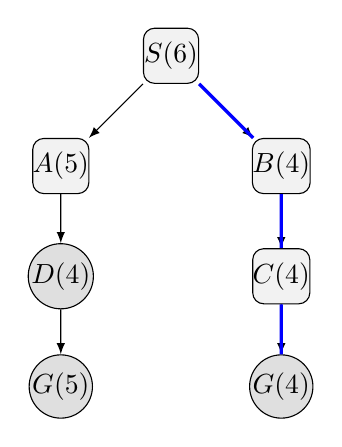
\begin{tikzpicture}[
            level distance=14mm,
            sibling distance=28mm,
            every node/.style={draw, circle, minimum size=7mm, inner sep=0pt},
            chosen/.style={draw, circle, fill=gray!25, minimum size=7mm, inner sep=0pt},
            edge from parent/.style={draw, -latex}
        ]
        \node[draw, rectangle, rounded corners, fill=gray!10] (S) {$S(6)$}
        child { node[draw, rectangle, rounded corners, fill=gray!10] (A) {$A(5)$}
                child { node[chosen] (D) {$D(4)$}
                        child { node[chosen] (G1) {$G(5)$} }
                    }
            }
        child { node[draw, rectangle, rounded corners, fill=gray!10] (B) {$B(4)$}
                child { node[draw, rectangle, rounded corners, fill=gray!10] (C) {$C(4)$}
                        child { node[chosen] (G2) {$G(4)$} }
                    }
            };
        \draw[very thick, blue] (S) -- (B) -- (C) -- (G2);
    \end{tikzpicture}
    \caption{Contoh pohon pencarian A$^\ast$. Jalur terpilih adalah $S \rightarrow B \rightarrow C \rightarrow G$ karena kombinasi biaya aktual $g(n)$ dan heuristik $h(n)$ menghasilkan nilai $f(n)$ terkecil.}
    \label{fig:contoh-astar}
\end{figure}

Pada contoh ini, A$^\ast$ tidak hanya melihat kedekatan ke tujuan, tetapi juga biaya yang sudah ditempuh. Karena itu, jalur yang dipilih bisa berbeda dari GBFS dan lebih terarah menuju solusi optimal dibandingkan pencarian berbasis heuristik murni.

\section{Heuristik yang Digunakan}
Pada implementasi solver ini, tersedia beberapa heuristik yang dapat dipilih untuk dipakai pada algoritma A$^\ast$ maupun GBFS. Masing-masing heuristik dirancang untuk memberi estimasi jarak atau biaya yang berbeda terhadap posisi tujuan.

\begin{enumerate}
    \item \textbf{ManhattanToTarget}

          Heuristik ini menghitung jarak Manhattan dari posisi aktor saat ini ke titik tujuan \texttt{O}. Jika posisi aktor adalah $(x_1, y_1)$ dan tujuan berada pada $(x_2, y_2)$, maka
          $$h(n) = |x_1 - x_2| + |y_1 - y_2|.$$
          Heuristik ini sederhana dan cepat dihitung, sehingga cocok sebagai estimasi awal. Untuk A$^\ast$, nilai ini dapat dikalikan dengan biaya minimum tile agar lebih sesuai dengan fungsi cost.

    \item \textbf{RemainingPlusManhattan}

          Heuristik ini menggabungkan dua komponen, yaitu jumlah checkpoint/angka yang masih tersisa untuk dilewati dan jarak Manhattan ke target berikutnya. Secara intuitif, semakin banyak angka yang belum dilewati, semakin besar nilai heuristiknya. Bentuk sederhananya dapat ditulis sebagai
          $$h(n) = \alpha \cdot r(n) + \beta \cdot d_{manhattan}(pos(n), target(n)),$$
          dengan $r(n)$ adalah jumlah checkpoint yang tersisa, $target(n)$ adalah target yang harus dicapai berikutnya, dan $\alpha, \beta$ adalah bobot pengali.

    \item \textbf{WeightedRemainingToGoal}

          Heuristik ini memberi bobot lebih besar pada sisa checkpoint dan jarak menuju tujuan akhir. Dibandingkan heuristic sebelumnya, pendekatan ini lebih agresif karena mendorong pencarian untuk segera menyelesaikan urutan checkpoint sebelum fokus penuh ke tujuan akhir. Bentuk umumnya adalah
          $$h(n) = \gamma \cdot r(n) + \delta \cdot d_{manhattan}(pos(n), goal),$$
          dengan $\gamma$ dan $\delta$ sebagai bobot. Heuristik ini berguna jika ingin pencarian lebih terarah, tetapi perlu diuji agar tetap memberikan perilaku yang stabil pada berbagai papan.
\end{enumerate}

Secara umum, heuristik pertama lebih ringan dan sederhana, sedangkan dua heuristik lainnya mencoba memasukkan informasi progres permainan, yaitu jumlah checkpoint yang belum dilewati. Pemilihan heuristik bergantung pada tujuan pencarian, apakah lebih mengutamakan kecepatan komputasi, jumlah node yang diekspansi, atau kualitas solusi yang ditemukan.

\subsection{Admissibility Heuristik}
\begin{itemize}
    \item \textbf{ManhattanToTarget}: pada bentuk yang dipakai sebagai estimasi jarak murni, heuristik ini dapat dianggap \emph{admissible} selama ia hanya memberikan batas bawah terhadap biaya sisa. Dalam implementasi yang memperhitungkan cost tile, bentuk yang paling aman adalah $d_{manhattan}(pos(n), goal) \times c_{min}$, dengan $c_{min}$ sebagai cost tile terkecil pada papan. Jika hanya memakai Manhattan tanpa pengali cost minimum, heuristik tersebut tetap cenderung menjadi batas bawah pada jumlah langkah, tetapi belum tentu merepresentasikan batas bawah cost secara ketat pada papan dengan bobot tile yang bervariasi.

    \item \textbf{RemainingPlusManhattan}: heuristik ini \textbf{tidak dijamin admissible}. Alasannya, komponen jumlah checkpoint tersisa $r(n)$ dan bobot $\alpha, \beta$ dapat membuat estimasi lebih besar dari biaya sisa yang sebenarnya. Begitu heuristik mulai menambahkan penalti untuk checkpoint secara agresif, nilai $h(n)$ berpotensi melebihi cost minimum menuju solusi.

    \item \textbf{WeightedRemainingToGoal}: heuristik ini juga \textbf{tidak dijamin admissible}. Penggunaan bobot $\gamma$ dan $\delta$ membuat estimasi semakin fleksibel, tetapi sekaligus meningkatkan risiko overestimate. Heuristik ini lebih cocok dipakai sebagai heuristik \emph{informed} untuk mempercepat pencarian, bukan untuk menjamin optimalitas A$^\ast$.
\end{itemize}

Dengan demikian, jika tujuan utama adalah menjaga optimalitas A$^\ast$, heuristik yang paling aman dipakai adalah ManhattanToTarget dalam bentuk batas bawah cost. Sebaliknya, dua heuristik berbobot lebih cocok digunakan pada GBFS atau pada mode A$^\ast$ ketika optimalitas tidak menjadi prioritas utama.

\section{Komparasi Teoretis Algoritma Pencarian}

\subsection{Kriteria perbandingan}
Perbandingan didasarkan pada beberapa kriteria teoritis yang sering dipakai dalam analisis algoritma pencarian, yaitu
\begin{itemize}
    \item \textbf{Kompleksitas waktu}: jumlah node yang mungkin diekspansi sebagai fungsi branching factor $b$ dan kedalaman solusi $d$.
    \item \textbf{Kompleksitas memori}: ukuran frontier dan struktur data yang disimpan (sering menjadi batas praktis utama pada pencarian graf/ruang keadaan besar).
    \item \textbf{Kelengkapan (completeness)}: apakah algoritma menjamin menemukan solusi bila ada.
    \item \textbf{Optimalitas (optimality)}: apakah algoritma menjamin solusi biaya minimum menurut fungsi cost yang didefinisikan.
    \item \textbf{Ketergantungan pada heuristik}: bagaimana kualitas/jenis heuristik memengaruhi performa dan jaminan teori.
\end{itemize}

\subsection{Properti Algoritma}
\begin{itemize}
    \item \textbf{Uniform-Cost Search (UCS)}
          \begin{itemize}
              \item Kompleksitas waktu: dalam kasus terburuk, ekspansi bisa $O(b^{\lceil C^*/\epsilon\rceil})$ di mana $C^*$ adalah biaya solusi optimal dan $\epsilon$ adalah cost min positif pada edge; secara intuitif sangat sensitif terhadap rentang dan nilai cost.
              \item Kompleksitas memori: menyimpan seluruh frontier dan explored set (sering eksponensial pada $d$).
              \item Kelengkapan: lengkap jika semua edge cost $\ge 0$ dan graf tidak memuat siklus dengan cost negatif.
              \item Optimalitas: menjamin optimalitas biaya jika semua edge cost non-negatif.
              \item Heuristik: tidak memerlukan heuristik; tidak mendapat keuntungan dari informasi heuristik.
          \end{itemize}

    \item \textbf{Greedy Best-First Search (GBFS)}
          \begin{itemize}
              \item Kompleksitas waktu: sangat bergantung pada kualitas heuristik; dalam analisis kasar, dapat mendekati $O(b^d)$ jika heuristik menyesatkan, tetapi sering jauh lebih sedikit node diekspansi bila heuristik informatif.
              \item Kompleksitas memori: menyimpan frontier (biasanya lebih kecil dari UCS/A$^\ast$ pada kasus yang heuristiknya sangat informatif), tetapi masih bisa besar bila heuristik buruk.
              \item Kelengkapan: tidak selalu lengkap pada ruang keadaan dengan branching tak terbatas; pada graf finite biasanya lengkap jika implementasi menangani revisits, tetapi tidak ada jaminan teoretis umum.
              \item Optimalitas: tidak optimal  GBFS hanya mengejar nilai heuristik terkecil tanpa mempertimbangkan biaya yang sudah dikeluarkan.
              \item Heuristik: performa sangat sensitif terhadap akurasi heuristik; heuristik admissible/consistent tidak memberi jaminan optimalitas untuk GBFS.
          \end{itemize}

    \item \textbf{A$^\ast$}
          \begin{itemize}
              \item Kompleksitas waktu: secara teoretis antara UCS dan GBFS; node yang diekspansi bergantung pada seberapa informatif heuristik $h$. Semakin mendekati biaya sisa sebenarnya, semakin sedikit node yang diekspansi.
              \item Kompleksitas memori: menyimpan frontier dan explored set sama seperti UCS  bisa menjadi faktor pembatas utama.
              \item Kelengkapan: lengkap jika heuristic dan struktur graf memenuhi asumsi standar (mis. finite branching dan biaya edge non-negatif).
              \item Optimalitas: A$^\ast$ menjamin optimalitas jika heuristik \emph{admissible} (tidak overestimate) dan biasanya memerlukan konsistensi (monotonicity) agar implementasi dengan pruning sederhana tetap benar.
              \item Heuristik: kualitas heuristik menentukan efektivitas; heuristik admissible tapi lebih informatif (lebih tinggi namun dari cost sebenarnya) mengurangi ekspansi signifikan.
          \end{itemize}
\end{itemize}

\subsection{Perbandingan Teoretis}
\begin{itemize}
    \item \textbf{Admissibility vs. Konsistensi}: admissibility ($h(n) \le h^*(n)$) penting untuk optimalitas A$^\ast$. Konsistensi (monotonicity) memastikan bahwa nilai $f$ pada frontier tidak menurun dan memungkinkan implementasi tanpa perlu reprocessing node yang sudah diekspansi.

    \item \textbf{Pengaruh branching factor $b$ dan kedalaman $d$}: banyak analisis asymptotic didasarkan pada $b$ dan $d$. Ketika $b$ besar dan $d$ juga besar, biaya waktu dan memori tumbuh eksponensial sehingga teknik penghematan memori (IDA$^\ast$, search with limited memory) perlu dipertimbangkan.

    \item \textbf{Trade-off waktu vs memori}: UCS dan A$^\ast$ umumnya menukar memori untuk waktu (menyimpan frontier besar untuk menghindari rekalkulasi), sedangkan variasi seperti IDA$^\ast$ menurunkan memori dengan biaya waktu tambahan.

    \item \textbf{Kualitas heuristik}: heuristik yang lebih informatif (lebih dekat ke biaya sisa nyata) mengurangi jumlah node yang diekspansi, namun jika heuristik meng-overestimate (non-admissible), A$^\ast$ kehilangan jaminan optimalitas. GBFS memilih agresivitas heuristik di atas semua, sehingga sangat cepat bila heuristik akurat tetapi sangat berisiko bila heuristik menyesatkan.

\end{itemize}

